\section{Порождающая модель}
\label{sec:gen}

Все пять таблиц --- наблюдения над одним объектом: кривой доза-эффект для тройки «молекула $m$,
фермент $e$, плечо $a$» (плечо --- прямое измерение или измерение после преинкубации). Модель
описывает эту кривую, а не отдельные таблицы, и каждая таблица подключается своим
правдоподобием.

Слово «правдоподобие» здесь ключевое и дальше встречается постоянно, поэтому стоит сказать,
что за ним стоит. Настоящей кривой мы не видим никогда --- видим только результаты измерений,
каждое со своим шумом. Правдоподобие отвечает на вопрос: если предположить, что настоящая
кривая вот такая, насколько ожидаемым было бы то, что мы на самом деле намерили? Обучение
состоит в переборе возможных кривых в пользу тех, при которых наблюдения выглядят наименее
удивительно. Записывают это обычно через $-\log p$ --- логарифм берут, чтобы вероятности
разных измерений складывались, а не перемножались, а минус --- чтобы задача стала задачей
минимизации. Ценность такой записи в том, что каждый источник данных добавляет в общую сумму
своё слагаемое, и разные по природе измерения оказываются на одном языке.

Латентные параметры тройки:
\begin{equation}
\theta_{m,e,a} = (\pi_{m,e,a},\; E_{m,e,a},\; h_e),
\qquad
\pi_{m,e,\text{tdi}} = \pi_{m,e,\text{dir}} + \Delta_{m,e} .
\label{eq:theta}
\end{equation}

Здесь $\pi$ --- потенция, та самая $\pic$; $E$ --- предельная глубина подавления, то есть какая доля
активности фермента подавляется при бесконечной концентрации; $h$ --- крутизна перехода, вынесенная
на уровень фермента (почему --- в разделе~\ref{sec:ident}).

Сдвиг $\Delta$ по химии неотрицателен: преинкубация может только усилить ингибирование, а не
ослабить. В данных предпосылка выполняется, и всё же \emph{ограничение не накладывается}. Жёсткое
$\Delta \ge 0$ доведено до кода и измерено на четырёх разбиениях: ранг падает на всех четырёх
ферментах, тогда как та же вторая голова без ограничения нейтральна. Прежняя редакция несла
неравенство прямо в определении \eqref{eq:theta}; оно оттуда убрано, потому что это не свойство
модели, а гипотеза, которая проверена и отвергнута. Разбор --- в разделе~\ref{sec:neg}.

Прямая модель прибора --- доля подавленной активности при концентрации $C$:
\begin{equation}
I(C;\theta) = \frac{E}{1 + 10^{\,h(\pC - \pi)}},
\qquad \pC = -\log_{10} C .
\label{eq:hill}
\end{equation}

Уравнение Хилла. При $\pC = \pi$, то есть когда концентрация равна IC$_{50}$, показатель обнуляется
и подавлена ровно половина от предельной глубины. Выше концентрация --- меньше $\pC$ --- отрицательнее
показатель --- ближе $I$ к $E$. Ниже --- наоборот. Крутизна $h$ задаёт, за сколько декад концентрации
происходит переход: при $h = 1$ путь от десяти до девяноста процентов эффекта занимает примерно две декады.

\subsection{Правдоподобия по источникам}

Кривая из двенадцати точек даёт несимметричную оценку: интервал вокруг $\pic$ обычно длиннее с одной
стороны. Усреднять границы --- терять эту информацию, поэтому порождающая модель задаёт расщеплённую нормаль с двумя
масштабами:
\begin{equation}
-\log p(y_{\text{крив}} \mid \pi)
= \operatorname{split-}\!\mathcal{N}(\pi;\, \hat\pi,\, \sigma^-,\, \sigma^+),
\qquad
\sigma^- = \frac{\hat\pi - l}{1.96},\quad \sigma^+ = \frac{h - \hat\pi}{1.96} .
\label{eq:split}
\end{equation}

Две половинки нормального распределения с разными ширинами, сшитые в моде и отнормированные общим
множителем $2/[\sqrt{2\pi}(\sigma^-+\sigma^+)]$. Правило деления на 1.96 точно только при симметричной
полосе: у расщеплённой нормали слева лежит масса $\sigma^-/(\sigma^-+\sigma^+)$, а не половина, поэтому
квантиль стоит не в 1.96 сигмы. На наших данных полосы почти симметричны --- максимум медианной асимметрии
0.13 логарифмической единицы --- и расхождение составляет 0.0004 единицы $\pic$. Правило годится, но
по этой причине, а не по общей верности.

\emph{И вся эта спецификация измерена, и она проигрывает.} Расщеплённая нормаль как обучающая цель
доведена до кода и прогнана на четырёх разбиениях против квадратичной потери, в двух углах: сама по
себе и поверх мёртвой зоны раздела~\ref{sec:deadzone}.

\begin{center}
\begin{tabular}{lcc}
\toprule
цель & ST-RAE & ранг \\
\midrule
квадратичная                    & 0.7204 & 0.5615 \\
расщеплённая нормаль            & 0.8106 & 0.5098 \\
квадратичная + мёртвая зона     & 0.6835 & 0.5955 \\
расщеплённая нормаль + мёртвая зона & 0.7252 & 0.5680 \\
\bottomrule
\end{tabular}
\end{center}

$-0.0517$ ранга сама по себе, минус на всех четырёх ферментах, и $-0.0275$ поверх мёртвой зоны. Два
угла нужны были потому, что одно сравнение с квадратичной не отличило бы «помогает асимметрия» от
«помогает полоса», --- и ответ ни то ни другое: жёсткий допуск несёт информацию полосы целиком, а
градуированный вес не добавляет к нему ничего и сам по себе отнимает.

Описание данных при этом верное: полосы действительно асимметричны, и усреднение границ действительно
теряет информацию. Неверным оказался переход от описания к обучающей цели.

Скрининг входит через \eqref{eq:hill} с аффинной калибровкой на фермент:
\begin{equation}
\hat y_{\text{скр}} = s_e \cdot \log_2\bigl(1 - I(C_0;\theta_{\text{dir}})\bigr) + b_e,
\qquad
-\log p(y_{\text{скр}} \mid \theta,\psi_e)
= \frac{(y_{\text{скр}} - \hat y_{\text{скр}})^2}{2(\sigma_i^2 + \sigma_e^2)} + \log\sqrt{\sigma_i^2+\sigma_e^2}.
\label{eq:scr}
\end{equation}

Прибор показывает логарифм оставшейся активности, отсюда $\log_2(1-I)$. Пара $(s_e, b_e)$ поглощает
динамический диапазон пробы и нормировку; $\sigma_i$ --- опубликованная стандартная ошибка конкретного
измерения, $\sigma_e$ --- обучаемая добавка, отвечающая за неучтённый разброс. Набор
$\psi_e = (s_e, b_e, \sigma_e)$ и есть калибровка прибора.

Emax --- прямое наблюдение второго параметра тройки; плечо с преинкубацией --- наблюдение $\pi + \Delta$
с тем же расщеплённым нормальным правдоподобием.

Ни расщеплённая нормаль, ни плечо с преинкубацией в подачу не вошли, и оба по измерению, а не по
недосмотру. Расщеплённая нормаль --- см. выше. Плечо вторым выходом при свободной $\Delta$ нейтрально,
с ограничением $\Delta \ge 0$ вредит, а точное правило раздела~\ref{sec:decision},
проинтегрированное по совместному распределению, улучшает калибровку втрое и ухудшает различение.
Три способа употребить одно и то же второе условие, и ни один не платит; почему так --- в
разделе~\ref{sec:ident}, подраздел о бюджете идентифицируемости.

\subsection{Калибровка прибора}
\label{sec:calib}

Калибровка --- это функция, переводящая скрытую кривую в показание прибора. Не свойство соединения,
а свойство установки: та же молекула на другом приборе даст другое показание, а $\pic$ у неё останется
прежней. Связь нелинейная и насыщающаяся: очень сильный ингибитор и ингибитор вдесятеро сильнее дадут
при 49.5 мкМ практически одинаковое показание, потому что оба подавили всё, что можно.

Подгоняем $E$ и $h$ на фермент по соединениям, у которых есть и то и другое измерение.

\begin{figure}[htbp]\centering
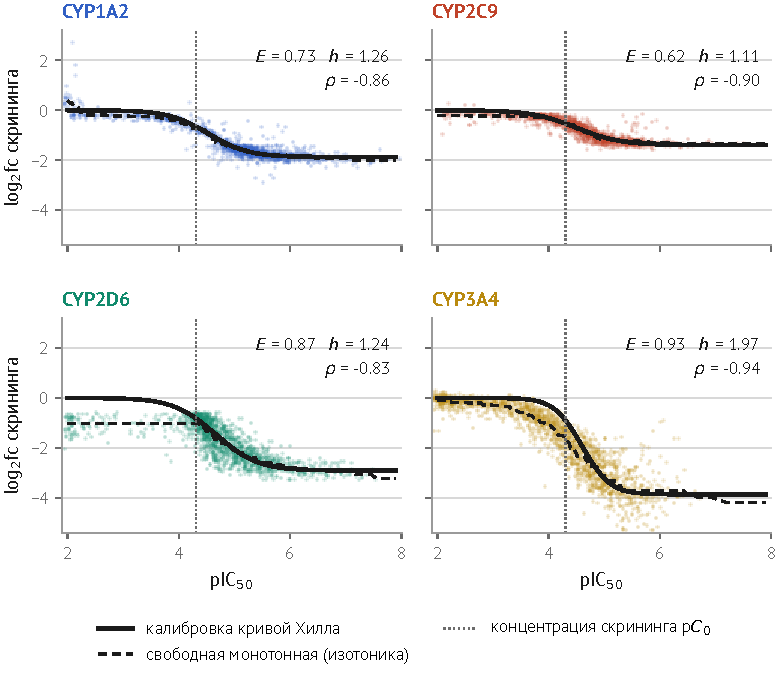
\includegraphics{fig/calib}
\caption{Калибровка. Точки --- соединения, у которых есть и $\pic$, и показание скрининга. Сплошная
линия --- подгонка формой \eqref{eq:hill} с двумя параметрами на фермент, пунктир --- свободная
монотонная кривая, задающая предел для любой монотонной калибровки.}
\label{fig:calib}
\end{figure}

Из этой картинки следует три вещи.

Связь очень сильная: ранговая корреляция от $-0.83$ до $-0.94$. Поэтому скрининг --- почти достаточная статистика. Свободная монотонная калибровка по \emph{измеренному} показанию даёт макро-ST-RAE
0.359 против 0.767 у полной модели по структуре. Знай мы показание скрининга для тестовых соединений,
задача была бы вдвое легче; но на тесте его нет, пересечение теста с первичной библиотекой ровно нулевое.

Хилловская форма теряет немного, но теряет. Стандартное отклонение остатка против свободной монотонной
кривой: 0.231 против 0.208 на 1A2, 0.185 против 0.167 на 2C9, 0.497 против 0.390 на 2D6, 0.612 против
0.499 на 3A4. То есть двухпараметрическая форма жёстче, чем нужно, особенно на 2D6, где свободная кривая
выходит на плато у неактивных, а хилловская тянется к нулю. Это аргумент за монотонную сплайн-поправку
поверх параметрической формы, но не за отказ от неё: форма даёт правильную экстраполяцию там, где данных мало.

Крутизна разная: на 3A4 подобралось $h = 1.97$, на остальных около 1.2. Это свойство постановки
на конкретном ферменте, поэтому калибровка не может быть общей на все четыре.

И этого мало. На CYP3A4 одна пара $(E, h)$ не описывает даже ту популяцию, на которой подогнана:
если расколоть скринированный набор пополам по уровню метки и подогнать каждую половину отдельно,
крутизна выходит 0.503 на нижней и 2.516 на верхней --- пятикратный размах \emph{внутри одного
фермента}, шире всего межферментного разброса. Перенос констант одной половины на другую стоит там
+1.365 против +0.019\ldots+0.067 у остальных трёх. Что за этим стоит --- в разделе~\ref{sec:ident}.

Отдельно проверен планшетный дрейф. Планшетов девять на фермент, и сырой разброс медиан по планшетам
выглядит тревожно: до 0.293 при размахе 0.922. Но планшеты не рандомизированы, активные соединения сидят
кучно, поэтому надо вычесть то, что объясняется составом планшета. После вычитания предсказанного
по $\pic$ разброс падает до 0.039--0.087 при стандартном отклонении остатка 0.19--0.61.

Планшет объясняет от 0.9 до 8 процентов остаточной дисперсии, и разброс по ферментам здесь важнее
диапазона: 3A4 0.9\,\%, 2D6 2.3\,\%, 1A2 3.2\,\%, а 2C9 8.1\,\% --- почти в девять раз больше, чем 3A4.
Вычитание свободной монотонной калибровкой вместо хилловской даёт 0.9, 2.7, 3.8 и 6.7 процента, то есть
та же картина: число --- свойство данных, а не выбора калибровки. Отдельного слагаемого в модели всё же
не требуется, но по другой причине, чем малость доли: даже на 2C9 планшетная компонента даёт
стандартное отклонение около 0.05 в единицах $\log_2$fc, что заметно меньше собственной погрешности
одного показания.

Про обозначение: $E$ в калибровке --- не тот $E$, что в \eqref{eq:theta}. Там предельная
глубина подавления самого соединения, здесь --- параметр установки, вбирающий её динамический диапазон.
Совпадение буквы неудачное и в коде их надо развести.

\subsection{Почему цензурирование получается само}
\label{sec:cens}

Это главный технический аргумент за такую конструкцию. Продифференцируем \eqref{eq:hill} по потенции,
обозначив $x = 10^{h(\pC_0 - \pi)}$:
\begin{equation}
\frac{\partial I}{\partial \pi}
= + E\, h \ln 10 \cdot \frac{x}{(1+x)^2} .
\label{eq:dI}
\end{equation}

Множитель $x/(1+x)^2$ максимален при $x = 1$, то есть ровно когда $\pi = \pC_0$, и равен там одной
четвёртой; при $x \to 0$ и $x \to \infty$ он затухает экспоненциально. Фишеровская информация о $\pi$,
которую несёт одна точка скрининга, пропорциональна квадрату этого множителя.

\begin{figure}[htbp]\centering
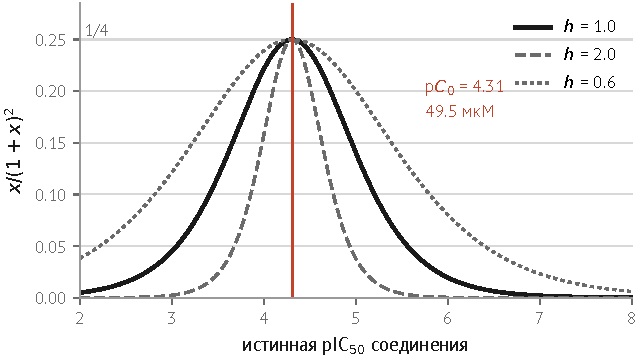
\includegraphics{fig/fisher}
\caption{Сколько информации о потенции несёт одно измерение при концентрации $C_0$. Колокол сосредоточен
вокруг $\pC_0$ с шириной порядка $1/h$ декад и обнуляется в обеих зонах насыщения.}
\label{fig:fisher}
\end{figure}

На практике это значит, что в зонах насыщения градиент по $\pi$ исчезает сам. Для соединения, которое при
49.5 мкМ не подавило ничего, модель извлекает из скрининга мягкое неравенство «активность ниже примерно
такой-то», а не число. Для соединения, подавившего всё, --- неравенство с другой стороны. Никакого
специального кода цензурирования писать не надо, оно следует из формы кривой.

Форма \eqref{eq:dI} видна в данных напрямую: перегиб зависимости показания от $\pic$ на CYP3A4 приходится
на 4.3 (рис.~\ref{fig:calib}), то есть на $\pC_0 = 4.305$ для 49.5 мкМ.
